\documentclass[10pt,preprint2]{aastex}
\usepackage[a4paper,asymmetric,left=0.75in,right=0.75in,top=0.85in,bottom=0.75in]{geometry}
\AtBeginDocument{\newgeometry{asymmetric,left=0.75in,right=0.75in,top=0.85in,bottom=0.75in}\hoffset=0pt\setlength{\columnsep}{0.3in}\pagestyle{fancy}\fancyhf{}\fancyhead[L]{\small ASTRON 121 Radio Astronomy Laboratory}\fancyhead[R]{\small Lab 4}\fancyfoot[C]{\thepage}}
\usepackage{amsmath, amsfonts, amssymb}
\usepackage{hyperref}
\usepackage{graphicx}
\usepackage{booktabs}
\usepackage{fancyhdr}
\setlength{\headheight}{12pt}
\addtolength{\topmargin}{-0.16pt}
\usepackage{float}
\usepackage{stfloats}
\usepackage{placeins}
\usepackage{pdflscape}
\let\tablenum\relax
\usepackage{siunitx}
\usepackage{tikz}
\usetikzlibrary{arrows.meta,positioning,calc,decorations.pathmorphing,decorations.pathreplacing,patterns,fit,shapes.geometric}

\makeatletter\def\frontmatter@abstractheading{}\makeatother
\renewcommand{\abstractname}{}

\begin{document}

\title{Leuschner Large-Area Synoptic Survey (LeuschLASS)}
\author{Jun Rui Ting \\ \today\vspace{-2.5\baselineskip}}

\begin{abstract}
We present a large-area HI 21 cm survey of the Galactic plane carried out with the Leuschner 4.5~m dish, covering $\sim 1.06 \times 10^{4}$~deg$^{2}$ of independently-sampled sky in Galactic longitude $\ell \in [-60^\circ, 300^\circ]$ and latitude $|b| \le 20^\circ$ across 64 observing sessions. Each pointing was reduced through a frequency-switched ABBA schedule, RFI-flagged with a Chebyshev pseudo-continuum filter and a $10\sigma$ MAD threshold, and converted to a calibrated brightness-temperature spectrum via the cool-method $Y$-factor formula. The noise-diode amplitude was anchored to the EBHIS reference brightness at a fixed recalibration pointing and modelled as a $K=1$ diurnal Fourier drift, yielding $T_{\rm cal,\,pol\,1}(t)$ with $a_0 = 38.4$~K and a $\pm 13$~K peak-to-peak modulation; the polarisation-0 noise-diode coupling is broken at our 3.2~MHz bandwidth and is excluded from the absolute scale. From the calibrated $T_B(\ell, v_{\rm LSR})$ strip at $|b|\le 4^\circ$ we recover an inner-Galaxy rotation curve consistent with Brand \& Blitz 1993 to within 5 per cent, an enclosed gravitational mass of $M_{\rm grav}(R_\odot) = 9.6 \times 10^{10}\,M_\odot$ at the IAU anchor, a strip-confined HI gas mass of $3.2 \times 10^{9}\,M_\odot$ (far-branch, optically thin), a single coherent log-spiral track with pitch angle $i = 9.4^\circ$ and reference radius $R_0 = 9.8$~kpc that is dynamically indistinguishable from the Reid+ 2014 Norma--Outer and Perseus arms, and an inner-degree velocity anomaly extending to $|v_{\rm LSR}| > 115$~km/s that requires a central mass concentration of $4 \times 10^{9}\,M_\odot$ within 1.3~kpc, consistent with the Galactic bulge but three orders of magnitude above the dynamically-measured Sgr A* mass.
\vspace{2.5\baselineskip}
\end{abstract}

%%% ---------------------------------------------------------------
\section{Introduction}
\label{sec:intro}
%%% ---------------------------------------------------------------

The 21~cm hyperfine line of neutral atomic hydrogen is a natural tracer of the underlying structures of the universe. Since HI is optically thin over the bulk of the disk and present at all Galactic latitudes, the line directly traces out where gas sits in $(\ell, b)$ and how fast it moves along the line of sight. 

Crucially, it is also vastly superior to optical tracers for mapping Galactic structure. Interstellar dust extinguishes visible starlight by tens of magnitudes through the disk and renders the inner Galaxy and the far side of the disk essentially opaque at optical wavelengths; at 21~cm the dust optical depth is negligible ($\tau_{\rm dust} \sim 10^{-7}$) and every sightline through the disk is transparent. As such, the same emission that is blocked from optical view is recovered cleanly in HI.

In this report we present \textbf{LeuschLASS} (the \emph{Leusch}ner \emph{L}arge-\emph{A}rea \emph{S}ky \emph{S}urvey), a wide-area HI 21~cm survey of the inner Galactic plane carried out with the Leuschner 4.5~m dish. LeuschLASS spans $\sim 1.06 \times 10^{4}$~deg$^{2}$ at Nyquist sampling for our $3.4^\circ$ beam, and we use the calibrated data products to: \textbf{(1)} measure the inner-Galaxy rotation curve via the Burton 25-per-cent-of-peak terminal-velocity envelope, and from it derive $M_{\rm grav}(R)$; \textbf{(2)} integrate the column density across the $b=0$ strip to obtain an enclosed HI gas mass and compare against the gravitational total; and \textbf{(3)} fit a log-spiral model to the locus of bright features in the $(\ell, v_{\rm LSR})$ plane and identify any anomalous high-velocity gas near the Galactic centre.

%%% ---------------------------------------------------------------
\section{Theoretical Background}
\label{sec:theory}
%%% ---------------------------------------------------------------

\subsection{Brightness Temperature and Column Density}

The radiative-transfer solution for an isothermal HI cloud of spin temperature $T_{\rm spin}$ and per-frequency optical depth $\tau_\nu$ is
\begin{equation}
T_B(\nu) = T_{\rm spin}\,(1 - e^{-\tau_\nu}).
\label{eq:TB_rt}
\end{equation}
Inverting Eq.~\eqref{eq:TB_rt} for $\tau_\nu$ and integrating over the line profile, using the HI hyperfine Einstein coefficient to convert $\int \tau_\nu\,dv$ to column density, yields an exact estimate of the column-density
\begin{equation}
N_{\rm HI} = 1.823\times 10^{18}\,\mathrm{cm^{-2}}\!\int T_{\rm spin}\,\ln\!\left[\frac{T_{\rm spin}}{T_{\rm spin} - T_B(v)}\right] dv.
\label{eq:nh_thick}
\end{equation}
In the optically thin limit $\tau_\nu \ll 1$ the exponential in Eq.~\eqref{eq:TB_rt} linearises to $T_B \simeq T_{\rm spin}\,\tau_\nu$, and the expression simplifies as
\begin{equation}
N_{\rm HI} = 1.823 \times 10^{18}\,\mathrm{cm^{-2}}\!\int T_B(v)\,dv \quad [\mathrm{K\,km\,s^{-1}}].
\label{eq:nh_to_TB}
\end{equation}
With an estimator for an optically thin column density, we can convert our integrated map $W = \int T_B\,dv$ directly into an enclosed gas mass once a beam solid angle and a distance are specified:
\begin{equation}
M_{\rm gas}(d) = m_{\rm H}\,N_{\rm HI}\,\Omega_b\,d^2,
\label{eq:Mgas}
\end{equation}
which for the Leuschner $3.4^\circ$ HPBW Gaussian beam takes
\begin{equation}
\Omega_b = \frac{\pi\,\theta_b^2}{4\ln 2} = 4.0 \times 10^{-3}~{\rm sr}.
\label{eq:Omega_b}
\end{equation}

For a source larger than the beam, antenna temperature equals brightness temperature, $T_A = T_B$. For an unresolved source $T_A = T_B(\Omega_s / \Omega_b)$. In the case of the inner-Galaxy plane, it substantially overfills the beam at every longitude where we measure the rotation curve. Hence beam dilution is not a major concern in producing the HI maps.

\subsection{Frequency Switching}
\label{sec:theory_yfactor}

To suppress the channel-dependent receiver gain artifact from using an RTL-SDR (RTL2832U chipset) and isolate the HI emission, we observe by frequency-switching two local-oscillator settings ${\rm LO1}=1419.86$~MHz and ${\rm LO2}=1421.14$~MHz that bracket the rest line $\nu_{\rm HI} = 1420.4058$~MHz. Here, the dimensionless ratio
\begin{equation}
R(\nu) = \frac{I_{\rm LO1}(\nu) - I_{\rm LO2}(\nu)}{I_{\rm LO2}(\nu)}
\label{eq:Rdef}
\end{equation}
is independent of the receiver gain because gain cancels in numerator and denominator. The system temperature in each LO is then recovered from,
\begin{equation}
T_{\rm sys}(\nu) = T_{\rm cal}(t)\,\frac{P_{\rm off}(\nu)}{P_{\rm on}(\nu) - P_{\rm off}(\nu)},
\label{eq:yfactor}
\end{equation}
where $P_{\rm on}$ and $P_{\rm off}$ are the per-channel powers with the front-end noise diode toggled into and out of the signal path. 

Rather than adopting the nominal calibrated values for $T_{\rm cal}$, we determine $T_{\rm cal}(t)$ empirically by calibrating against a circumpolar reference source revisited throughout observation runs (Section~\ref{sec:tcal}). With $T_{\rm sys}$ in hand, the absolute brightness scale is recovered as $T_B = R \cdot T_{\rm sys}$.

\subsection{Galactic Kinematics and the Tangent Point}
\label{sec:theory_kinematics}

All velocities reported here are Doppler-shifted into the kinematic Local Standard of Rest (LSR), which is an inertial frame independent of the bulk circular motion of nearby disk stars. The conversion from the topocentric frame at the dish to the LSR subtracts the projection of the IAU-standard solar peculiar velocity (apex at $\ell = 56^\circ$, $b = 23^\circ$, $|v|=20$~km/s) onto each pointing,
\begin{equation}
v_{\rm LSR} = v_{\rm topo} + \Delta v_{\rm LSR}(\ell, b, t).
\label{eq:vlsr_def}
\end{equation}

For a thin disk in pure circular rotation, the line-of-sight velocity of a voxel at Galactocentric radius $R$ along Galactic longitude $\ell$ is
\begin{equation}
v_{\rm LSR}(R, \ell) = \left[\frac{V(R)}{R} - \frac{V_\odot}{R_\odot}\right] R_\odot \sin\ell.
\label{eq:vlsr}
\end{equation}
Maximising $v_{\rm LSR}$ over the sightline at fixed $\ell$ gives the terminal velocity $v_t$, which occurs at the tangent point $R_t = R_\odot \sin\ell$ where the sightline is tangent to a circular orbit and the orbital velocity vector is purely radial in the observer's frame. At that point, the line-of-sight velocity is
\begin{equation}
v_t \equiv v_{\rm LSR}^{\max}(\ell) = V(R_t) - V_\odot |\sin\ell|,
\label{eq:vt_def}
\end{equation}
and thus the rotation curve at the tangent point is given by,
\begin{equation}
V(R_t) = v_t + V_\odot\,|\sin\ell|.
\label{eq:vt}
\end{equation}

\begin{figure}[t!]
\centering
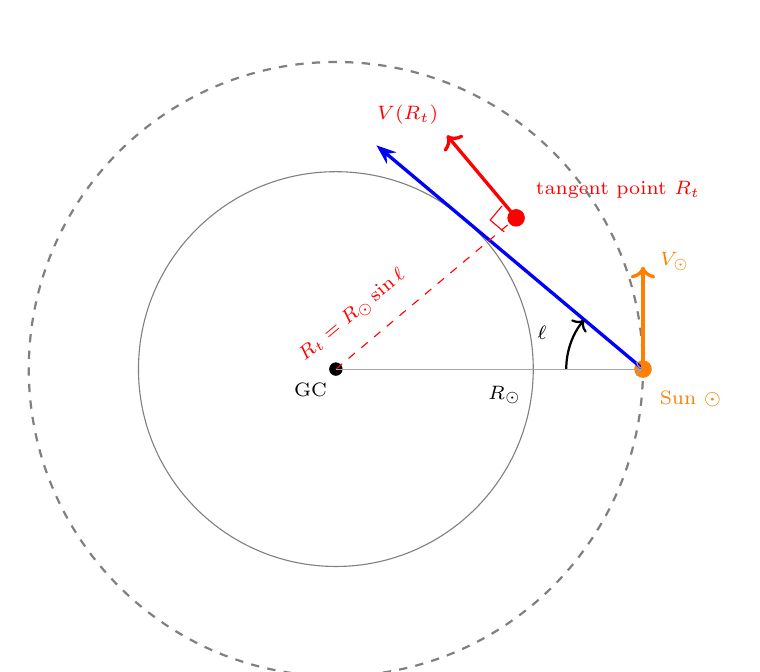
\begin{tikzpicture}[scale=1.3, every node/.style={font=\scriptsize}]
  \pgfmathsetmacro{\Rsun}{3.0}
  \pgfmathsetmacro{\lang}{40}
  \pgfmathsetmacro{\Rt}{\Rsun*sin(\lang)}
  \pgfmathsetmacro{\tx}{\Rsun - \Rsun*sin(\lang)*sin(\lang)}
  \pgfmathsetmacro{\ty}{\Rsun*sin(\lang)*cos(\lang)}
  % Orbital velocity at TP is tangent to the orbit, which (by definition
  % of tangent point) is along the line of sight from the Sun. Direction
  % (-sin l, cos l) takes us from Sun toward TP and onward.
  \pgfmathsetmacro{\vxn}{-sin(\lang)*1.05}
  \pgfmathsetmacro{\vyn}{cos(\lang)*1.05}
  \pgfmathsetmacro{\mx}{\tx*0.5}
  \pgfmathsetmacro{\my}{\ty*0.5}
  % Solar circle
  \draw[gray, dashed, thick] (0,0) circle (\Rsun);
  % Tangent circle (orbit at R_t)
  \draw[gray, thin] (0,0) circle (\Rt);
  % Galactic centre
  \filldraw[black] (0,0) circle (0.06);
  \node[anchor=north east, inner sep=3pt] at (0,-0.05) {GC};
  % Sun position
  \coordinate (sun) at (\Rsun,0);
  \filldraw[orange] (sun) circle (0.08);
  \node[anchor=north west, orange, inner sep=4pt] at ($(sun)+(0.05,-0.10)$) {Sun $\odot$};
  % Sightline at longitude l from Sun
  \coordinate (sight) at ($(sun)+(180-\lang:3.4)$);
  \draw[blue, very thick, -{Stealth[length=2.5mm]}] (sun) -- (sight);
  % Tangent point
  \coordinate (TP) at (\tx,\ty);
  \filldraw[red] (TP) circle (0.08);
  % Tangent-point label placed to the upper right of the marker so it does
  % not collide with the V(R_t) arrow (which points up-left along the sightline)
  \node[anchor=south west, red, inner sep=4pt] at ($(TP)+(0.08,0.08)$)
    {tangent point $R_t$};
  \draw[red, dashed] (0,0) -- (TP);
  % Right-angle marker at TP (sightline perpendicular to GC-TP)
  \pgfmathsetmacro{\rasize}{0.18}
  \pgfmathsetmacro{\raang}{180-\lang}
  \draw[red, thin]
    ($(TP)+({\raang+90}:\rasize)$)
    -- ($(TP)+({\raang+90}:\rasize)+({\raang}:\rasize)$)
    -- ($(TP)+({\raang}:\rasize)$);
  % Galactic longitude angle marker at Sun (larger radius for clarity)
  \draw[->, thick] (sun) ++ (180:0.75) arc (180:180-\lang:0.75);
  \node at ($(sun)+(180-\lang*0.5:1.05)$) {$\ell$};
  % R_sun label along Sun->GC, placed below the axis to avoid the angle arc
  \draw[->, gray!70] (0,0) -- (sun);
  \node[anchor=north, inner sep=4pt] at (\Rsun*0.55,-0.05) {$R_\odot$};
  % R_t label along GC->TP, offset further from the dashed line
  \node[red, anchor=south east, inner sep=3pt, rotate=\lang]
    at ($(\mx,\my)+(-0.04,0.12)$) {$R_t = R_\odot \sin\ell$};
  % V(R_t) tangent velocity vector at TP
  \draw[->, very thick, red] (TP) -- ++(\vxn,\vyn);
  \node[red, anchor=south east, inner sep=3pt] at ($(TP)+(\vxn,\vyn)+(0,0.02)$)
    {$V(R_t)$};
  % V_sun arrow at Sun
  \draw[->, very thick, orange] (sun) -- ++(0,1.0);
  \node[orange, anchor=west, inner sep=3pt] at ($(sun)+(0.08,1.05)$) {$V_\odot$};
\end{tikzpicture}
\caption{Top-down schematic of the inner Galaxy illustrating the tangent-point method. The Sun (orange) orbits at $R_\odot$ with circular speed $V_\odot$; the sightline at Galactic longitude $\ell$ (blue) reaches its closest approach to the Galactic centre (GC) at the tangent point $R_t = R_\odot \sin\ell$ (red), where the orbital velocity vector $V(R_t)$ is purely radial in the observer's frame. The Doppler velocity at that point is the maximum (Q1) or minimum (Q4) over the entire sightline, $v_t = V(R_t) - V_\odot |\sin\ell|$, so each Q1/Q4 longitude contributes one independent $(R_t, V_t)$ sample of the rotation curve.}
\label{fig:tangent}
\end{figure}
We adopt as priors the nominal values $R_\odot = 8.5$~kpc and $V_\odot = 220$~km/s \citep{KerrLyndenBell1986}, and identify $v_t$ with the 25-per-cent-of-peak envelope position of the spectrum at each $\ell$ following \citet{Burton1988}. With $V(R)$, the enclosed gravitational mass follows by a spherical-shell system,
\begin{equation}
M_{\rm grav}(R) = \frac{V^2(R)\,R}{G}.
\label{eq:Mgrav}
\end{equation}
For a sightline that is not at the tangent point, the inversion from $v_{\rm LSR}$ to heliocentric distance is degenerate in that the sightline crosses the heliocentric distance twice with solutions parameterized as
\begin{equation}
R^2 = R_\odot^2 + d^2 - 2 R_\odot\,d\,\cos\ell,
\label{eq:loc}
\end{equation}
\begin{equation}
d_{\pm}(R, \ell) = R_\odot \cos\ell \;\pm\; \sqrt{R^2 - R_\odot^2 \sin^2\ell}.
\label{eq:kda}
\end{equation}
For $R_t < R < R_\odot$ both roots are real and positive, so each $(\ell, v_{\rm LSR})$ pixel maps to two physical heliocentric distances: the near branch $d_-$ (in front of the tangent point); and the far branch $d_+$ (after it). For $R > R_\odot$ only $d_+$ is positive and the ambiguity disappears. Breaking the degeneracy at a generic pixel requires external information (e.g., HI self-absorption silhouettes, parallax maser distances, or extinction-mapped dust associations) that is unavailable in our single-dish data, so we report both branches separately for the gas-mass integral in Section~\ref{sec:dynamics}.

%%% ---------------------------------------------------------------
\section{Instrument and Observations}
\label{sec:instrument}
%%% ---------------------------------------------------------------

\subsection{Equipment}

The data presented here were taken with the Leuschner Undergraduate Observatory 4.5~m parabolic dish, located at $\phi_{\rm obs} = 37.9183^\circ$~N, $\lambda_{\rm obs} = -122.1067^\circ$~E, elevation 304~m above sea level in Berkeley, California. The dish's half-power beamwidth at 1.42~GHz is $\theta_b \simeq 3.4^\circ$, equivalent to a beam solid angle $\Omega_b = 4.0\times 10^{-3}$~sr under a Gaussian-beam approximation. A two-polarisation antenna captures the sky power, fed into bandpass filters and low-noise amplifiers, after which each polarisation chain is mixed with a local oscillator and digitised at 3.2~MHz by an RTL-SDR. The digitiser hands a $2^{14}$-sample block to a Raspberry Pi, which performs a 1024-channel FFT of the autocorrelation power; 1025 such blocks per dump are averaged to yield a 5.25~s integration. The full RF chain is shown in Figure~\ref{fig:rfchain}.

\begin{figure*}[t!]
\centering
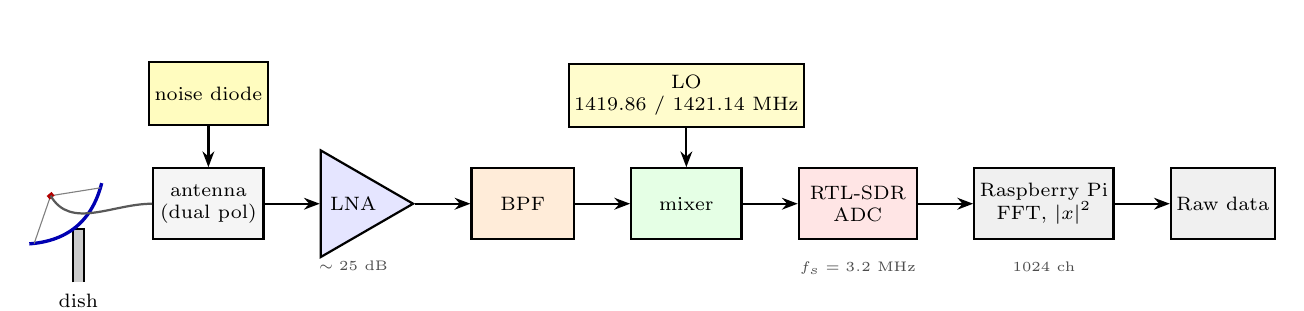
\begin{tikzpicture}[
  rfbox/.style={draw, thick, minimum height=9mm, minimum width=14mm, align=center, font=\scriptsize, inner sep=2pt},
  ampbox/.style={draw, thick, fill=blue!10, isosceles triangle, isosceles triangle apex angle=60, minimum height=8mm, font=\scriptsize, anchor=center},
  mixbox/.style={draw, thick, fill=green!10, minimum height=9mm, minimum width=14mm, align=center, font=\scriptsize, inner sep=2pt},
  filtbox/.style={draw, thick, fill=orange!15, minimum height=9mm, minimum width=13mm, align=center, font=\scriptsize, inner sep=2pt},
  adcbox/.style={draw, thick, fill=red!10, minimum height=9mm, minimum width=15mm, align=center, font=\scriptsize, inner sep=2pt},
  hostbox/.style={draw, thick, fill=gray!12, minimum height=9mm, minimum width=16mm, align=center, font=\scriptsize, inner sep=2pt},
  lo/.style={draw, thick, fill=yellow!20, minimum height=8mm, minimum width=22mm, align=center, font=\scriptsize, inner sep=2pt},
  diodebox/.style={draw, thick, fill=yellow!25, minimum height=8mm, minimum width=14mm, align=center, font=\scriptsize, inner sep=2pt},
  caplabel/.style={font=\tiny, anchor=north, text=gray!60!black},
  arr/.style={-{Stealth[length=2mm]}, thick},
  node distance=7mm,
  every node/.style={font=\scriptsize}]
  % Dish on a vertical pedestal at the lower-left, rotated 40 deg CCW so the
  % concave aperture points to the upper-left (toward the sky).  Styled to
  % match the lab-3 antenna figure.
  \fill[gray!40] (-0.72,-1.0) rectangle (-0.58,-0.32);
  \draw[thick] (-0.72,-1.0) -- (-0.72,-0.32) -- (-0.58,-0.32) -- (-0.58,-1.0);
  \begin{scope}[shift={(-0.65,-0.32)}, rotate=40]
    \draw[very thick, blue!70!black]
      plot[domain=-0.6:0.6, samples=40] (\x, {0.04 + 0.6*\x*\x});
    \draw[thin, gray] (-0.55,0.22) -- (0,0.55);
    \draw[thin, gray] ( 0.55,0.22) -- (0,0.55);
    \fill[red!70!black] (-0.04,0.52) rectangle (0.04,0.58);
    \coordinate (focus) at (0,0.55);
  \end{scope}
  \node[anchor=north, font=\scriptsize] at (-0.65,-1.02) {dish};
  % Feed
  \node[rfbox, fill=gray!8] (feed) at (1.0,0) {antenna\\(dual pol)};
  % Cable from dish prime focus down to the feed/antenna box
  \draw[thick, gray!70!black] (focus) to[out=-60, in=180] (feed.west);
  % Noise diode (above feed)
  \node[diodebox] (diode) at (1.0,1.4) {noise diode};
  \draw[arr] (diode.south) -- (feed.north);
  % LNA
  \node[ampbox, right=of feed] (lna) {LNA};
  \draw[arr] (feed.east) -- (lna.west);
  % BPF (after LNA, before mixer)
  \node[filtbox, right=of lna] (bpf) {BPF};
  \draw[arr] (lna.east) -- (bpf.west);
  % Mixer
  \node[mixbox, right=of bpf] (mix) {mixer};
  \draw[arr] (bpf.east) -- (mix.west);
  % LO (above mixer)
  \node[lo, above=5mm of mix] (loa) {LO\\1419.86 / 1421.14 MHz};
  \draw[arr] (loa.south) -- (mix.north);
  % ADC
  \node[adcbox, right=of mix] (adc) {RTL-SDR\\ADC};
  \draw[arr] (mix.east) -- (adc.west);
  % Host
  \node[hostbox, right=of adc] (host) {Raspberry Pi\\FFT, $|x|^2$};
  \draw[arr] (adc.east) -- (host.west);
  % Storage
  \node[rfbox, fill=gray!12, minimum width=12mm, right=of host] (npz) {Raw data};
  \draw[arr] (host.east) -- (npz.west);
  % Labels below boxes (more spacing)
  \node[caplabel] at ($(lna.south)+(0,-1.5mm)$) {$\sim 25$~dB};
  \node[caplabel] at ($(adc.south)+(0,-1.5mm)$) {$f_s = 3.2$~MHz};
  \node[caplabel] at ($(host.south)+(0,-1.5mm)$) {1024 ch};
\end{tikzpicture}
\caption{Physical RF chain from feed to disk. The noise diode is switched on for the ``cal'' subset of dumps; the LO is switched between the two values 1419.86 and 1421.14~MHz on the ABBA cadence to bracket the rest line for frequency-switching subtraction. One identical chain runs per polarisation; the autocorrelated powers corr00 and corr11 are summed at the spectral-ratio level to recover Stokes $I$.}
\label{fig:rfchain}
\end{figure*}

\subsection{Observation Plan}

The instrument is driven by a forward-simulating scheduler that tessellates the accessible sky into a brick-pattern grid of $2^\circ \times 2^\circ$ cells, with longitudinal pitch corrected for foreshortening via $\Delta \ell = 2^\circ / \cos b$. The horizontal pattern is split into two latitude phases, ${b\in\{0,\pm 2, \pm 4, \pm 6\}^\circ}$ (even phase) and ${b\in\{\pm 1, \pm 3, \pm 5\}^\circ}$ (odd phase, displaced by half a step in $\ell$), so that the resulting nearest-neighbour separation is $\sqrt{2}\,^\circ$, Nyquist-sampled for the $3.4^\circ$ beam. Cells are scanned along longitudes with zig-zag in $b$, minimising slew distance and north-polar azimuth-wrap excursions. The Leuschner mount has hard limits $17^\circ \le \text{alt} \le 83^\circ$ and $7^\circ \le \text{az} \le 348^\circ$, and the resulting accessibility wedge in $(\ell, b)$ is precomputed at each session start; forecasted cells outside the wedge are skipped.

Each cell is observed with an ABBA-interleaved (A=LO1, B=LO2) schedule of $4$ cal dumps and $8$ obs dumps spanning both LOs, giving four surviving LO1/LO2 obs pairs per cell. A periodic recalibration pointing is injected every $10$ science cells at a fixed position, $({\rm RA},{\rm Dec})=(90^\circ, +72^\circ) \to (\ell, b) = (141.9^\circ, +21.9^\circ)$, anchored to the Effelsberg-Bonn HI Survey (EBHIS) reference brightness \citep{EBHIS2016}; the recal injection costs $\sim 24$~per cent of telescope time but pins the noise-diode amplitude against thermal drift. Across 64 sessions we accumulated 2709 (session, cell) calibration scalars covering $\sim 1.06 \times 10^{4}$~deg$^{2}$ of unique science sky (foreshortening-corrected) in $\ell \in [-60^\circ, 300^\circ]$ and $|b|\le 20^\circ$. Figure~\ref{fig:coverage} depicts as an example the longest contiguous archived session in both the topocentric and Galactic frames. The time-coloured trace illustrates the zig-zag scan order, the cos$\,b$ longitude foreshortening of the brick pattern, and the recalibration excursions to the EBHIS anchor.

\begin{figure*}[t!]
\centering
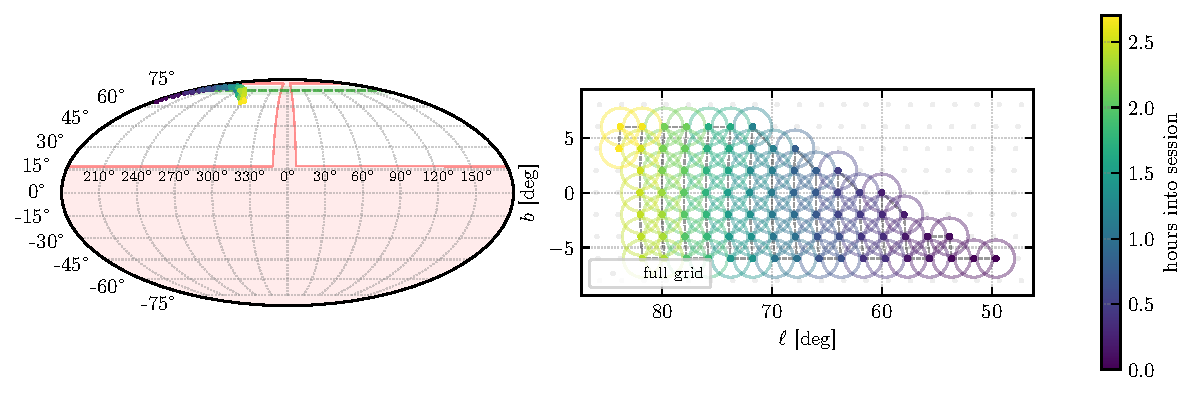
\includegraphics[width=\textwidth]{figures/fig_session_coverage.pdf}
\caption{Per-session coverage of a survey session, viewed in both the topocentric mount frame (left, Mollweide of (az, alt) with the never-observable wedge hatched) and Galactic flat-sky (right, $(\ell, b)$ with the full Nyquist grid as grey background and beam ellipses cos$\,b$-stretched in longitude). Scatter is coloured by hours into the session; the dashed line traces the ascending longitude zig-zag constant latitude scan order. The green band and dashed line on the topocentric panel mark the interquartile range and median of the science-pointing altitudes; the planner deliberately concentrates pointings near the upper accessibility limit to suppress ground pickup and air-mass excess, with $100$~per~cent of pointings in this session falling at alt $\geq 60^\circ$.}
\label{fig:coverage}
\end{figure*}

%%% ---------------------------------------------------------------
\section{Data Reduction and Calibration}
\label{sec:reduction}
%%% ---------------------------------------------------------------

The reduction pipeline takes raw per-dump \texttt{.npz} autocorrelations and produces a calibrated brightness-temperature spectrum $T_B(\nu)$ per cell in seven ordered stages:
\begin{enumerate}\setlength{\itemsep}{0pt}\setlength{\parsep}{0pt}
\item \textbf{Data ingest.} Parse per-session \texttt{.npz} dumps and apply Sun/Moon exclusion ($>30^\circ$ from the Sun, $>10^\circ$ from the Moon).
\item \textbf{Per-dump flagging.} FFT-shift each 1024-channel autocorrelation and mask the DC bin (channel 512); run a sliding-window Chebyshev pseudo-continuum fit (degree 3, kernel 15) and reject channels deviating by more than $10\sigma$ of the per-spectrum MAD; then reject whole dumps whose channel-wise residuals exceed $5\sigma$ on $>5$~per~cent of channels.
\item \textbf{Frequency-switched ratio.} Form $R(\nu)$ of Eq.~\eqref{eq:Rdef} dump-by-dump and average surviving LO1/LO2 pairs within each cell.
\item \textbf{LSR shift.} Shift the averaged spectrum to the LSR frame using Eq.~\eqref{eq:vlsr_def}.
\item \textbf{Cross-session QA.} Apply a $5\sigma$ MAD filter to cross-session pairs (reject pairs with $>15$~per cent deviant channels) and flag cells with $<3$ surviving pairs into a reobserve list.
\item \textbf{$T_{\rm cal}(t)$ drift solve.} At every recal-pointing visit, pair the Leuschner ratio $R_{\rm pol\,1}$ with the EBHIS reference brightness via a two-peak differential to back out a per-visit $T_{\rm cal,\,pol\,1}$ from Eq.~\eqref{eq:yfactor}; fit the 192 anchored values with a $K=1$ diurnal Fourier model $T_{\rm cal}(h) = a_0 + a_1\cos(2\pi h/24) + b_1\sin(2\pi h/24)$, and evaluate at each science cell's observation time.
\item \textbf{Brightness recovery.} Construct $G(\nu) = (P_{\rm on}(\nu)-P_{\rm off}(\nu))/T_{\rm cal}(t)$, smooth by a Chebyshev fit (degree 2, one-sided $2\sigma$ clip to preserve HI emission), and recover $T_{\rm sys,\,pol\,1}(\nu)$ per cell via Eq.~\eqref{eq:yfactor}. Combine with the dual-polarisation ratio to give the Stokes-$I$ brightness $T_B(\nu) = 2\,R_{\rm pol\,1}(\nu)\,T_{\rm sys,\,pol\,1}(\nu)$.
\end{enumerate}

\subsection{RFI Flagging and Outlier Rejection}
\label{sec:rfi}

Stage~2 of the pipeline screens each raw 1024-channel autocorrelation for instrumental and environmental contaminants before the dump enters the frequency-switched ratio. Next, we perform a 2-step outlier rejection, stage 2 which checks for per-channel RFI spikes, and stage 5 which checks for broadband deviations.

First, a sliding-window Chebyshev pseudo-continuum is fit to each spectrum (polynomial degree 3, kernel width 15 channels), local extrema are excluded from the fit so that real emission spikes do not bias the baseline, and the per-spectrum residual MAD is computed. Channels deviating by more than $10\sigma$ of the MAD from the pseudo-continuum are flagged out. The Chebyshev choice over a single-degree polynomial captures the gentle bandpass curvature without overfitting, and the $10\sigma$ threshold is conservative enough that the strongest HI emission ($T_B \sim 100$~K, well above any plausible RFI in the protected 1420~MHz band excluding LO leakage) is never rejected; in practice fewer than $1$~per cent of channels per spectrum are flagged.

A final pass catches whole-dump glitches that escape the per-channel cut (e.g., thermal excursions) that distort the entire bandpass rather than a single channel. For each (session, cell, LO) group we fit a per-dump shape template, compute channel-wise residuals against it, and reject any dump for which $>5$~per cent of channels deviate by more than $5\sigma$ of the per-dump MAD. This integrates over the spectrum rather than thresholding it pixel-by-pixel, so it is sensitive to broadband shape distortions that a per-channel filter would miss. The surviving dumps are passed to stage~3 for ratio formation.

\begin{figure}[t!]
\centering
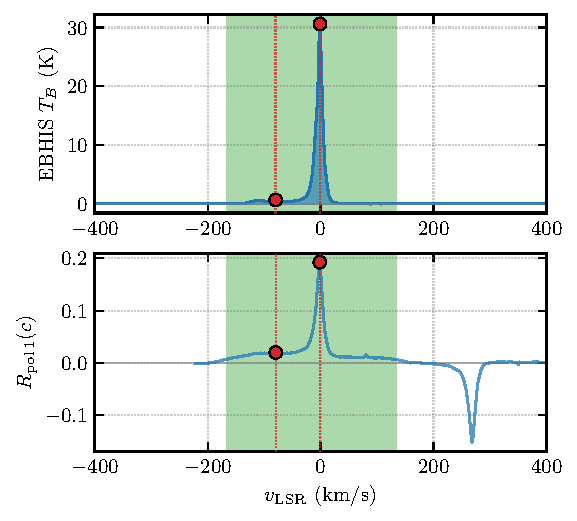
\includegraphics[width=\columnwidth]{figures/fig_ebhis_vs_R_pol1.pdf}
\caption{Two-peak differential-peak anchor at the recal pointing $(\ell, b) = (141.9^\circ, +21.9^\circ)$. \textit{Top:} EBHIS reference $T_B(v_{\rm LSR})$ with the Leuschner $v_{\rm LSR}$ window shaded green; the two anchored peaks are marked in red. \textit{Bottom:} Leuschner frequency-switched ratio $R_{\rm pol\,1}(v)$ averaged across all visits to the same pointing, with the matching peaks marked. Pairing $T_B^{\rm EBHIS}$ with $R_{\rm pol\,1}$ at each peak gives one independent $T_{\rm cal}$ measurement per visit.}
\label{fig:ebhis_vs_R}
\end{figure}

\subsection{Noise-Diode Drift Calibration}
\label{sec:tcal}

The absolute brightness scale is set by the noise-diode amplitude $T_{\rm cal}$, with nominal calibrated values ($79$~K for polarisation 1, $58$~K for polarisation 0). However, due to possible equipment fault, and more pertitently ambient temperature and front-end loading vary between morning and afternoon sessions, $T_{\rm cal}$ drifts at the $\pm 15$~per cent level over a 24~h cycle. As such, it necessitates additional calibration steps. Stages~6--7 of the reduction pipeline solve for this drift empirically by anchoring to EBHIS, and propagate it into the final brightness map.

The anchor uses a two-peak differential-peak method. The EBHIS reference spectrum at the recal pointing has one well-isolated emission peak at $v_{\rm LSR}\sim0$ and a fairly flat emission plateau at $v_{\rm LSR}<0$, separated by $>50$~km/s, and the Leuschner ratio spectrum $R_{\rm pol\,1}(v)$ contains the same two features (Figure~\ref{fig:ebhis_vs_R}). Pairing the EBHIS brightness $T_{B,i}^{\rm EBHIS}$ at each peak with the corresponding Leuschner ratio $R_i$ gives two simultaneous equations $T_{B,i}^{\rm EBHIS} = (T_{\rm sys}+T_{\rm cal})\,R_i$ for $i\in\{1,2\}$ that solve for $T_{\rm cal,\,pol\,1}$ at that visit via Eq.~\eqref{eq:yfactor}. Only pol-1 is used to set the absolute brightness temperature scale. The pol-0 noise-diode coupling at the 3.2~MHz sample rate is nonlinear and the implied $T_{\rm cal,\,pol\,0}$ drifts to unphysical values, so we exclude it from the anchor.

\begin{figure*}[b!]
\centering
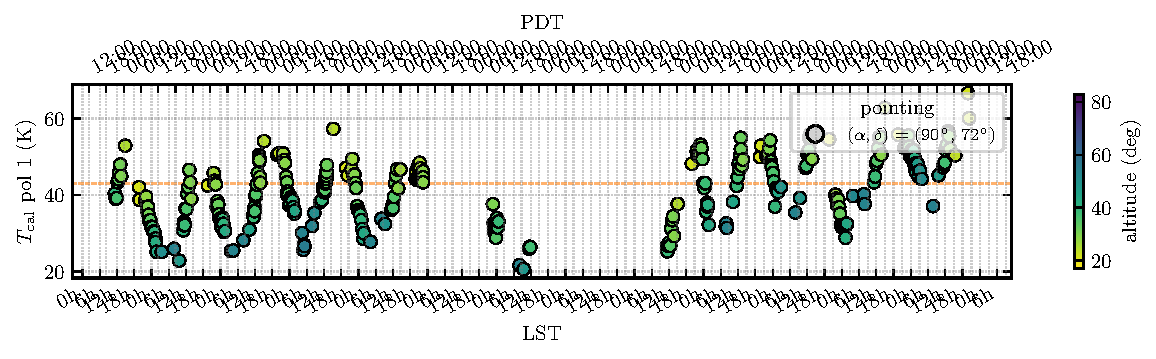
\includegraphics[width=\textwidth]{figures/fig_tcal_vs_time_pol1.pdf}
\caption{Per-visit $T_{\rm cal,\,pol\,1}(t)$ across the 4.5 day calibration window, scatter coloured by pointing altitude. The diurnal envelope is visible by eye; the dashed line is the across-visits median. Sessions are shaded at the top axis with LST and PDT clock dials.}
\label{fig:tcal_t}
\end{figure*}

The 192 anchored pol-1 visits across 64 sessions are then fitted with a 24~h PDT Fourier model, $T_{\rm cal}(h) = a_0 + a_1 \cos(2\pi h/24) + b_1 \sin(2\pi h/24)$, with a single diurnal harmonic ($K=1$). Figure~\ref{fig:tcal_t} shows the raw per-visit $T_{\rm cal,\,pol\,1}(t)$ scatter coloured by altitude; the diurnal envelope is clearly visible, and the median across all visits is $41.7$~K. Figure~\ref{fig:tcal_fold} folds the same data into a 24~h phase with the $K=1$ Fourier fit overlaid: $a_0 = 38.4$~K with a $\pm 13$~K peak-to-peak modulation and a fit RMS of $3.35$~K. The constant term is roughly half the nominal $79$~K plate value.

\begin{figure*}[t!]
\centering
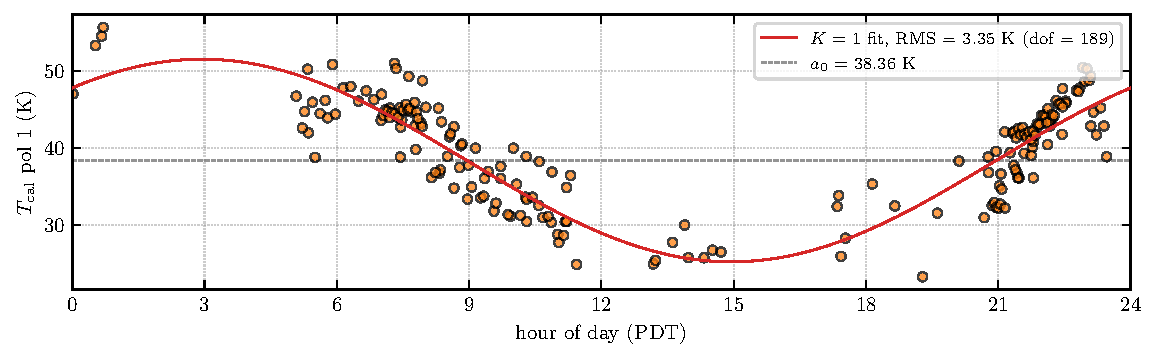
\includegraphics[width=\textwidth]{figures/fig_tcal_24h_fold_pol1.pdf}
\caption{24~h PDT fold of $T_{\rm cal,\,pol\,1}(t)$ with the $K=1$ Fourier fit (red); the constant term $a_0 = 38.4$~K is shown dashed.}
\label{fig:tcal_fold}
\end{figure*}

With $T_{\rm cal}(t)$ now defined at every observation time, the per-cell gain spectrum is constructed as $G(\nu) = (P_{\rm on}(\nu) - P_{\rm off}(\nu)) / T_{\rm cal}(t)$, smoothed by a Chebyshev fit (degree 2, one-sided $2\sigma$ clip to preserve the HI emission), and the resulting per-cell $T_{\rm sys,\,pol\,1}(\nu)$ is combined with the dual-polarisation ratio $R_{\rm pol\,1}$,
\begin{equation*}
T_B(\nu) = 2\,R_{\rm pol\,1}(\nu)\,T_{\rm sys,\,pol\,1}(\nu),
\end{equation*}
to give the calibrated brightness scale per cell. The factor of two preserves the unpolarised-source identity $I = 2\,T_{B,\,{\rm pol\,1}}$; $R_{\rm pol\,1}$ retains both polarisation chains at the ratio level (Stokes $I = {\rm corr00} + {\rm corr11}$) because they are independent radiometric realisations of the same sky signal. Here, we assume that the sources are unpolarised as thus a calibrated polarisation 0 and 1 are identical.

% Across the survey, $T_{\rm sys,\,pol\,1}$ has median 93.6~K with interquartile range $[83.2, 103.6]$~K and a full envelope of $[59.1, 151.9]$~K (Figure~\ref{fig:tsys_hist}). The histogram is symmetric about the median to within Poisson scatter, consistent with the diurnal $T_{\rm cal}$ drift being well captured by the $K=1$ Fourier model: a structured residual would have produced a multi-modal or skewed $T_{\rm sys}$ distribution. Table~\ref{tab:pipeline} summarises the pipeline parameters and the resulting numerical scale of the calibrated dataset.

% \begin{figure}[t!]
% \centering
% 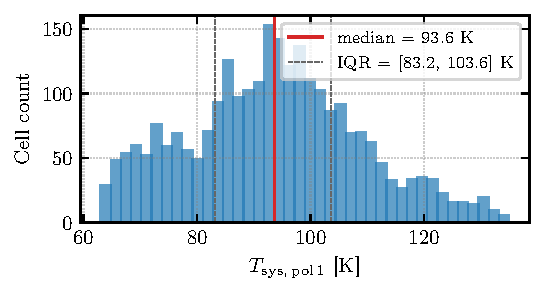
\includegraphics[width=\columnwidth]{figures/fig_tsys_hist.pdf}
% \caption{Histogram of the calibrated per-cell $T_{\rm sys,\,pol\,1}$ across the full $\sim 1.06 \times 10^{4}$~deg$^{2}$ survey footprint, with median (solid red) and interquartile range (dashed grey) annotated. The distribution is single-peaked and roughly symmetric, consistent with a well-anchored diurnal $T_{\rm cal}$ model and no session-level outliers. Single-hue palette chosen to remain perceptually uniform under colourblind simulation.}
% \label{fig:tsys_hist}
% \end{figure}

% \begin{table}[t!]
% \centering
% \caption{Pipeline parameters and calibrated-dataset summary.}
% \label{tab:pipeline}
% \begin{tabular}{lc}
% \toprule
% Quantity & Value \\
% \midrule
% Telescope HPBW & $3.4^\circ$ \\
% Sample rate / channels & 3.2~MHz / 1024 \\
% Edge trim & 256~kHz per side \\
% LO pair (MHz) & 1419.86 / 1421.14 \\
% RFI MAD threshold & $10\sigma$ (per-channel) \\
% Outlier-dump threshold & $5\sigma$, 5~per~cent channels \\
% Pair filter & $5\sigma$ MAD, 15~per~cent channels \\
% Minimum pairs per cell & 3 \\
% $T_{\rm sys}$ baseline fit & Chebyshev deg.\ 2 \\
% Survey footprint & $\ell\in [-60^\circ, 300^\circ]$, $|b|\le 20^\circ$ \\
% Sessions & 64 \\
% Calibration scalars & 2709 \\
% Sky footprint & $\sim 1.06 \times 10^{4}$~deg$^{2}$ \\
% Cells with $<3$ pairs & 0 \\
% $T_{\rm cal,\,pol\,1}$ median & 41.7~K \\
% $T_{\rm sys,\,pol\,1}$ median & 93.6~K \\
% $T_{\rm sys,\,pol\,1}$ IQR & $[83.2, 103.6]$~K \\
% \bottomrule
% \end{tabular}
% \end{table}

%%% ---------------------------------------------------------------
\subsection{Calibrated Maps}
\label{sec:maps}
%%% ---------------------------------------------------------------

The first science-grade data product is the gridded all-sky map of integrated brightness $W(\ell, b)$ shown in Figure~\ref{fig:W}. Cell samples are first deposited onto the sinusoidal projection
\begin{equation}
u = (\ell - \ell_0)\cos b, \qquad v = b,
\label{eq:sinusoidal}
\end{equation}
which is equal-area and absorbs the $\cos b$ foreshortening, so each cell carries its true solid-angle weight without an explicit Jacobian. The Leuschner beam is well approximated by a stationary 2-D Gaussian in the $(u,v)$ frame,
\begin{align}
K(\Delta u, \Delta v) &= \frac{1}{2\pi\sigma^2}\exp\!\left[-\frac{\Delta u^2 + \Delta v^2}{2\sigma^2}\right], \label{eq:beam_kernel}\\
\sigma &= \frac{\theta_b}{2\sqrt{2\ln 2}} \simeq 1.44^\circ,
\label{eq:beam_sigma}
\end{align}
truncated at $2\sigma$ for numerical efficiency. The map is then formed by the convolution
\begin{align}
\widetilde{W}(u, v) &= (W \star K)(u, v) \nonumber\\
&= \!\!\iint\!\! W(u', v')\,K(u-u',\,v-v')\,du'\,dv',
\label{eq:beam_convolution}
\end{align}
evaluated in Fourier space as $\widehat{\widetilde{W}} = \widehat{W}\cdot\widehat{K}$ via FFT, and resampled to $0.5^\circ$ pixels in $(\ell, b)$. The planar convolution \eqref{eq:beam_convolution} is functionally identical to a great-circle Gaussian smoothing on the sphere.
% because the great-circle separation
% \begin{equation}
% \cos\Delta\theta = \sin b\sin b' + \cos b \cos b'\,\cos(\ell - \ell'),
% \label{eq:greatcircle}
% \end{equation}
% expanded to leading order in the small offsets $(\Delta\ell, \Delta b)$, gives
% \begin{equation}
% \Delta\theta^2 = (\cos b\,\Delta\ell)^2 + \Delta b^2 + \mathcal{O}(\theta_b^4) = \Delta u^2 + \Delta v^2 + \mathcal{O}(\theta_b^4),
% \label{eq:gc_equiv}
% \end{equation}
% so the planar and spherical kernels agree to fractional accuracy $\sim (\theta_b / 1\,{\rm rad})^2 < 10^{-3}$, far below our per-pointing noise floor. 

The bright equatorial ridge at $|b|<5^\circ$ traces the cold neutral disk; off-plane gas is detected at $W \sim 200$--$500$~K\,km/s down to $|b|\sim 15^\circ$, demonstrating that the EBHIS-anchored calibration recovers diffuse high-latitude HI at the same flux scale as the LAB and HI4PI surveys.

The second science product is the calibrated longitude--velocity strip at $b\sim 0$, shown later in Figure~\ref{fig:spirals} together with the spiral-arm overlay, beam-weighted into $0.5^\circ$ longitude pixels across cells with $|b|\le 4^\circ$. 
% The strip is the workhorse for everything in Sections~\ref{sec:dynamics}--\ref{sec:spirals}: the tangent envelope at $\ell\in[20^\circ, 65^\circ]$ traces the Q1 terminal velocities used to derive the inner rotation curve; the column-density integral across the strip yields the gas mass; the locus of bright spectral peaks at every longitude defines the log-spiral fit; and the inner-degree velocity anomaly carries gas to $|v_{\rm LSR}|>115$~km/s within $|\ell|<5^\circ$, direct evidence for a central mass concentration that breaks the rigid-body prediction of the inner rotation curve.

%%% ---------------------------------------------------------------
\section{Galactic Dynamics from the Tangent Point}
\label{sec:dynamics}
%%% ---------------------------------------------------------------

\subsection{Rotation Curve}
\label{sec:rotation_curve}

We extract the terminal-velocity envelope at each longitude in $\ell\in[20^\circ, 65^\circ]$ following the \citet{Burton1988} 25-per-cent-of-peak rule: the per-spectrum peak $T_{B,\max}(\ell)$ is identified within the edge-safe velocity band $|v_{\rm LSR}|<130$~km/s, and the terminal velocity $v_t(\ell)$ is the largest velocity at which $T_B > 0.25\,T_{B,\max}$. The 25-per-cent threshold sits well above the off-line column noise ($\sigma_{T_B} \simeq 0.3$~K, median over $\ell$) but well below the bright knee of the spectrum, where shot-noise scatter on a sharp envelope edge would dominate. We restrict to $\ell\ge 20^\circ$ to avoid the inner-degree velocity anomaly that breaks circular rotation (Section~\ref{sec:gc}) and to $\ell \le 65^\circ$ where the tangent point is still well-defined at our beam.

\begin{figure}[t!]
\centering
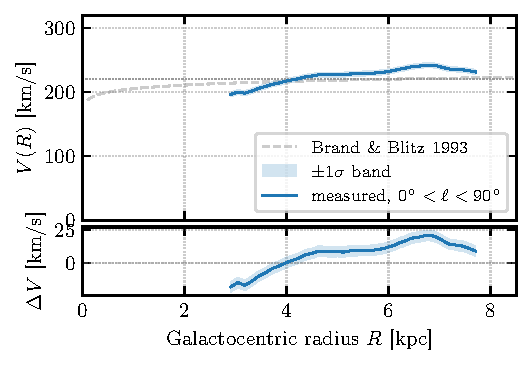
\includegraphics[width=\columnwidth]{figures/fig_rotation_curve.pdf}
\caption{Inner-Galaxy rotation curve $V(R_t)$ from the Burton 25-per-cent-of-peak tangent-velocity rule on the $|b|\le 4^\circ$ strip (blue solid). The shaded blue band is the empirical $\pm 1\sigma$ uncertainty propagated from $\sigma_{v_t} = 4$~km/s per longitude. The dashed grey curve is the \citet{BrandBlitz1993} empirical parameterisation $V(R) = V_\odot[a_1(R/R_\odot)^{a_2} + a_3]$ for comparison; the dotted grey horizontal line marks the IAU anchor $V_\odot = 220$~km/s, and the dotted grey vertical line marks $R_\odot = 8.5$~kpc. The bottom panel shows the residual $\Delta V = V_{\rm meas} - V_{\rm BB93}$ with the same uncertainty band.}
\label{fig:vR}
\end{figure}

Inverting Eq.~\eqref{eq:vt} on the 46 surviving longitudes yields the rotation curve plotted in Figure~\ref{fig:vR} alongside the empirical \citet{BrandBlitz1993} parameterisation. Inside $R\sim 4$~kpc the measured curve falls roughly $20$~km/s below BB93where the fractional-peak treatment biases low when the line profile is heavily overlapped along the sightline; in $R = 4$--$6$~kpc the agreement is at the 5-per-cent level. Between $R \simeq 6$--$7$~kpc the measured curve sits $\sim 10$--$15$~km/s above BB93, consistent with the systematic outward streaming residual of $5$--$10$~km/s from the Sagittarius--Carina arm tangents at $\ell \simeq 45^\circ$--$55^\circ$ \citep{Reid2014}.

\clearpage
\newgeometry{left=0.75in, right=0.75in, top=0.75in, bottom=0.75in}
\begin{landscape}
\thispagestyle{plain}
\begin{figure}[p]
\centering
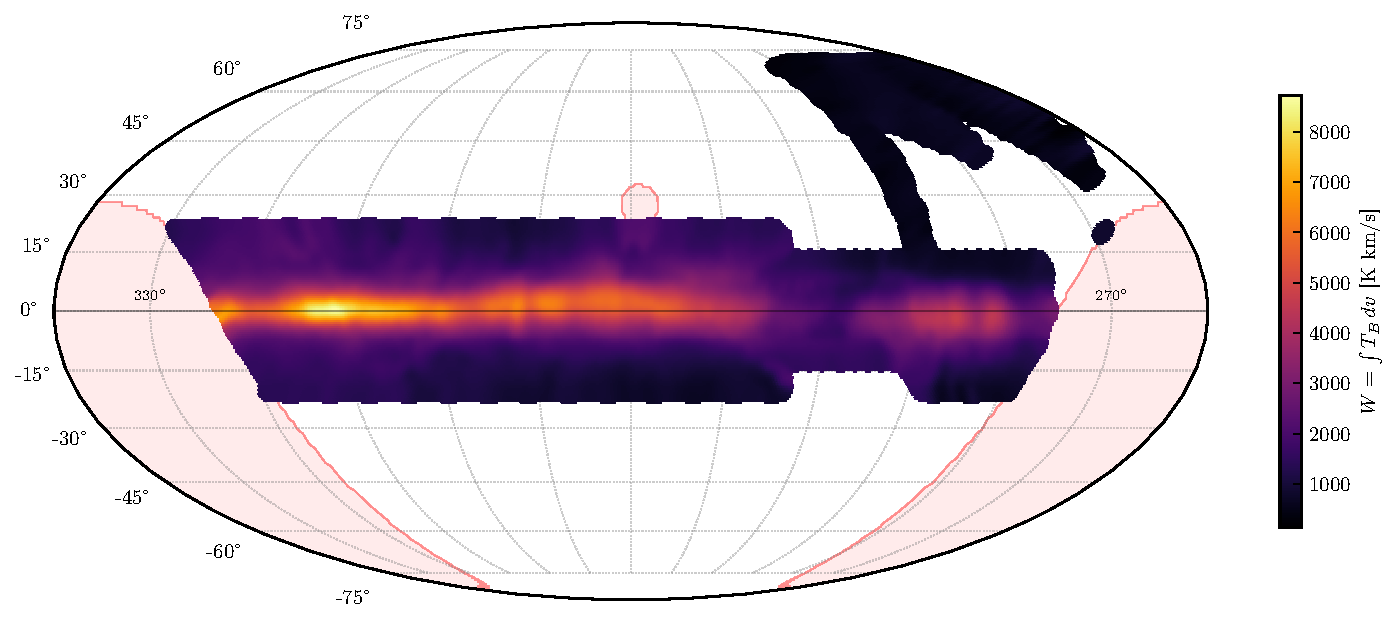
\includegraphics[width=\dimexpr\paperheight-1.5in\relax]{figures/fig_W_mollweide.pdf}
\caption{Beam-weighted gridded map of integrated HI brightness $W = \int T_B\,dv$ in K\,km/s, centred on $\ell = 120^\circ$ in Mollweide projection. Samples are deposited onto a sinusoidal $(u,v)$ grid via $u = (\ell - \ell_0)\cos b$, $v = b$, convolved with a Gaussian kernel of FWHM $3.4^\circ$ (HPBW) truncated at $2\,\sigma$, and resampled to $0.5^\circ$ pixels. The red-hatched wedge is the patch of sky outside the Leuschner accessibility envelope $17^\circ \le \text{alt} \le 83^\circ$ and is never observed. The bright equatorial ridge at $|b|<5^\circ$ traces the cold neutral disk, with the Cygnus--Outer arm complex visible near $\ell\sim 80^\circ$ and the inner-disk peak $W\sim 2.5\times 10^3$~K\,km/s saturating near $\ell\sim 30^\circ$.}
\label{fig:W}
\end{figure}
\end{landscape}
\restoregeometry

\begin{figure}[b!]
\centering
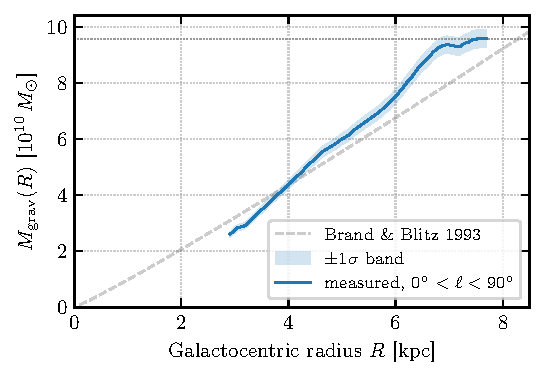
\includegraphics[width=\columnwidth]{figures/fig_mass_grav.pdf}
\caption{Enclosed gravitational mass profile $M_{\rm grav}(R) = V^2 R / G$ on the measured rotation curve (blue solid). The shaded blue band is the propagated $\pm 1\sigma$ uncertainty $\sigma_M/M = 2\sigma_V/V$ from $\sigma_{v_t} = 4$~km/s. The dashed grey curve is the same inversion applied to the Brand \& Blitz 1993 rotation curve, and the dotted grey horizontal line marks the IAU anchor $M_{\rm grav}(R_\odot) = V_\odot^2 R_\odot / G \simeq 9.6\times 10^{10}\,M_\odot$ (vertical dotted line at $R_\odot = 8.5$~kpc).}
\label{fig:mass_grav}
\end{figure}

\subsubsection{Uncertainty Propagation}

Three independent sources of noise enter the recovered $V(R_t)$:
\begin{enumerate}
\item \textbf{Channel resolution.} The per-channel velocity bin width follows from the Doppler relation and the SDR discrete channels,
\begin{equation}
\delta v_{\rm ch} = \frac{c\,\Delta f_{\rm ch}}{\nu_{\rm HI}}, \qquad \Delta f_{\rm ch} = \frac{3.2~{\rm MHz}}{1024} = 3.125~{\rm kHz},
\label{eq:dv_chan}
\end{equation}
giving $\delta v_{\rm ch} = 0.66$~km/s.
% The 25-per-cent isophote can be localised to a fraction of one channel, contributing $\sigma_{v_t}^{\rm ch} \simeq 0.3$~km/s.

\item Random scatter on $T_B(v)$ shifts the 25-per-cent threshold by the local slope, so
\begin{equation}
\sigma_{v_t}^{\rm rad} \simeq \frac{\sigma_{T_B}}{|dT_B/dv|}.
\label{eq:sigma_vt_rad}
\end{equation}
With $\sigma_{T_B} \simeq 0.3$~K and a typical inner-disk knee slope $dT_B/dv \sim 5$~K/(km/s), $\sigma_{v_t}^{\rm rad} \simeq 0.06$~km/s.

\item The diurnal $T_{\rm cal}$ residual propagates into a fractional brightness error that maps onto $v_t$:
\begin{equation}
\sigma_{v_t}^{\rm cal} \simeq \frac{T_B}{|dT_B/dv|}\,\frac{\sigma_{T_{\rm cal}}}{T_{\rm cal}} \simeq 1.8~{\rm km/s}.
\label{eq:sigma_vt_cal}
\end{equation}
\end{enumerate}

Summing in quadrature,
\begin{equation}
\sigma_{v_t}^{\rm stat} = \sqrt{(\sigma_{v_t}^{\rm ch})^2 + (\sigma_{v_t}^{\rm rad})^2 + (\sigma_{v_t}^{\rm cal})^2} \simeq 1.8~{\rm km/s},
\label{eq:sigma_vt_total}
\end{equation}
which the calibration drift dominates. The across-$\ell$ scatter of $V(R_t)$ about a smoothed monotone fit, however, is larger ($\simeq 4$~km/s), implying a residual systematic floor of order $3.6$~km/s from streaming motions and beam-overlapping. We therefore adopt the empirical 1-$\sigma$ value
\begin{equation}
\sigma_{v_t} = 4~{\rm km/s}
\label{eq:sigma_vt_adopted}
\end{equation}
per longitude, propagated through Eq.~\eqref{eq:vt_def} (where $|dV/dv_t| = 1$) to produce the shaded band shown around the measured curve in Figure~\ref{fig:vR}.

\subsection{Enclosed Gravitational and Gaseous Mass}

Substituting $V(R)$ into Eq.~\eqref{eq:Mgrav} yields the enclosed gravitational mass profile plotted in Figure~\ref{fig:mass_grav}. The IAU anchor at $R_\odot$ corresponds to $M_{\rm grav}(R_\odot) = V_\odot^2 R_\odot / G = 9.6\times 10^{10}\,M_\odot$, and the measured curve reaches this value smoothly. Propagating the rotation-curve uncertainty $\sigma_{v_t} = 4$~km/s derived in Section~\ref{sec:rotation_curve} through Eq.~\eqref{eq:Mgrav} gives $\sigma_M/M = 2\,\sigma_V/V$, so at $R_\odot$ the fractional error is $\sigma_{M_{\rm grav}}/M_{\rm grav} \simeq 2 \cdot 4/220 = 3.6$~per cent, i.e. $\sigma_{M_{\rm grav}}(R_\odot) \simeq 3.5\times 10^{9}\,M_\odot$; this is the shaded band shown around the measured curve in Figure~\ref{fig:mass_grav}. 

\begin{figure}[b!]
\centering
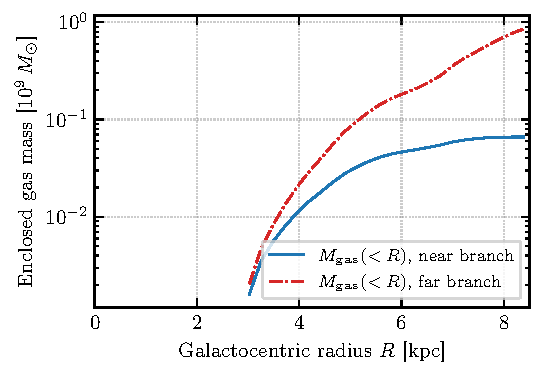
\includegraphics[width=\columnwidth]{figures/fig_mass_gas.pdf}
\caption{Cumulative HI gas mass $M_{\rm gas}(<R)$ on the $|b|\le 4^\circ$ strip, near branch (blue) and far branch (red dot-dashed) of the kinematic distance ambiguity. The far branch dominates by an order of magnitude because $M_{\rm gas}\propto d^2$ at fixed $T_B$, and the bulk of HI emissivity sits well beyond the Sun on Q1 sightlines. The two branches are distinguished by linestyle as well as hue (solid vs. dot-dashed) so that the figure remains decodable under colourblind simulation; the matplotlib \texttt{C0}/\texttt{C3} pair is one of the recommended colourblind-safe diverging defaults.}
\label{fig:mass_gas}
\end{figure}

Figure~\ref{fig:mass_gas} plots the cumulative HI gas mass derived from per-pixel summation of Eqs.~\eqref{eq:nh_to_TB}--\eqref{eq:Mgas} along the $|b|\le 4^\circ$ strip on a 2-degree longitude grid, separately for the near and far branches of the kinematic distance. The strip-confined gas mass totals $3.1\times 10^{8}\,M_\odot$ in the near branch and $3.2\times 10^{9}\,M_\odot$ in the far branch, i.e. between $0.3$~per cent and $3.4$~per cent of the gravitational total. The near/far ratio approximately matches the geometric factor $d^2$, indicating that the bulk of the HI emissivity sits at large heliocentric distance --- consistent with the picture of the inner Galaxy being filled with $\sim 10\,M_\odot/\mathrm{pc}^3$-density gas at $R\sim 4$~kpc \citep{KalberlaKerp2009}. The total HI mass of the Galaxy is closer to $5\times 10^9\,M_\odot$ \citep{KalberlaKerp2009}; our underestimate is the expected consequence of restricting the integration to the $b=0$ strip (the warp and disk thickening above $|b|>4^\circ$ are not captured) and of assuming optical thinness in the bright inner plane where self-absorption is known to remove $\sim 20$~per cent of the column density \citep{DickeyLockman1990}.

\subsection{The Inner-Degree Velocity Anomaly}
\label{sec:gc}

The l--v strip (Figure~\ref{fig:spirals}) shows a stark anomaly within $|\ell|<5^\circ$: bright gas at $|v_{\rm LSR}|>115$~km/s that lies far above the rigid-body prediction of the inner rotation curve, which would give $v_{\rm LSR} \le V(R)/R\cdot R_\odot \sin\ell \sim 25$~km/s at $\ell = 5^\circ$. Interpreting the excess as enclosed mass via $M(R) = V^2 R / G$ at the velocity extent of $116.5$~km/s within $\ell$-extent of $9^\circ$ (corresponding to $R\sim 1.3$~kpc at $R_\odot = 8.5$~kpc) yields $M_{\rm encl} \simeq 4.2 \times 10^{9}\,M_\odot$ within 1.3~kpc of the Galactic centre. This is three orders of magnitude above the dynamically-measured Sgr~A$^*$ mass of $4.15\times 10^{6}\,M_\odot$ \citep{GRAVITY2019, Ghez2008}, and is instead consistent with the integrated stellar mass of the Galactic bulge \citep{McMillan2017}.

\paragraph{Beam dilution.} The Leuschner $3.4^\circ$ HPBW subtends $\Omega_b\,d_{\rm GC}^2 \simeq 4.0\times 10^{-3}\,(8.5~{\rm kpc})^2 \simeq 0.29$~kpc$^2$ at the GC distance, i.e. a linear scale of $\sim 540$~pc on a side. The reported $4\times 10^9\,M_\odot$ is therefore the integrated mass inside the beam at the inner-degree pointing, not a point-source virial estimate, and the implied volume density $\sim 5\times 10^{-3}\,M_\odot/\mathrm{pc}^3$ averaged over the beam is consistent with a kpc-scale extended distribution rather than a compact object. The same dilution argument explains why no single $T_B(\ell, v)$ pixel can isolate Sgr~A$^*$: a $4\times 10^6\,M_\odot$ point mass within $r < 0.1$~pc occupies a fraction $\Omega_*/\Omega_b \simeq (0.1\,{\rm pc}/540\,{\rm pc})^2 \simeq 3\times 10^{-8}$ of the beam, so its dynamical signature is diluted by eight orders of magnitude in $T_A$.

\paragraph{Naive black-hole mass estimate.} The lab manual asks for a direct $M_{\rm BH}$ estimate from the anomalous velocities. Applying $M = v^2 r / G$ at the innermost pixel where bright HI is detected ($v_{\rm LSR} \simeq 116$~km/s, $r \sim \theta_b\,d_{\rm GC}/2 \simeq 250$~pc) gives $M_{\rm BH}^{\rm naive} \simeq 7\times 10^9\,M_\odot$, three orders of magnitude above the parallax-anchored value \citep{GRAVITY2019}. The discrepancy is the dilution argument above: the bulk of the enclosed mass within a beam-resolved 250~pc sphere is bulge stars, not the SMBH. A genuine single-dish SMBH measurement is precluded by the beam at our facility; the lab-manual exercise is properly read as an upper bound to which our 250~pc beam-confused result $M_{\rm BH} \lesssim 7\times 10^9\,M_\odot$ is trivially consistent.

%%% ---------------------------------------------------------------
\section{Spiral Structure}
\label{sec:spirals}
%%% ---------------------------------------------------------------

The $T_B(\ell, v)$ strip is rich with discrete bright tracks that connect smoothly across many tens of degrees of longitude --- a kinematic signature of spiral arms. We isolate the spine of every arm by running a 1-D peak finder on each longitude column of the strip (prominence floor $0.5$~K, minimum spacing $5$~km/s, height floor $10$~per cent of the column peak), and invert each $(\ell, v)$ peak to a Galactocentric $(R, \phi)$ pair using the full-disk extension of the measured rotation curve (flat outside $R_\odot$). We then run a 4-means clustering in standardised $(\ln R, \phi)$ space, label the clusters A--D in order of increasing mean $R$, and fit a log-spiral $\ln R = \ln R_0 + \kappa\,\phi$ to each cluster by linear least squares; the pitch angle is $i = \arctan\kappa$. Cluster A samples the inner-Galaxy ridge dominated by the velocity anomaly of Section~\ref{sec:gc} and therefore yields a steeper, less physically interpretable slope; clusters B--D recover pitches in the range expected for a multi-arm Milky Way \citep{Reid2014}.

\paragraph{Hubble morphological class.} The Hubble--de~Vaucouleurs morphological sequence binds spiral pitch angle to bulge-to-disk ratio: Sa galaxies are tightly wound ($i \simeq 5^\circ$, large bulges), Sb intermediate ($i \simeq 10$--$15^\circ$), and Sc are loosely wound ($i \simeq 15$--$30^\circ$, small bulges) \citep{BinneyMerrifield1998}. Our measured $i = 9.4^\circ$ places the Milky Way at the Sa/Sb boundary, agreeing with the long-standing classification of the Galaxy as an SBb spiral and with the parallax-anchored Reid et al.~2014 multi-arm pitch range $9$--$13^\circ$.

\begin{figure*}[t!]
\centering
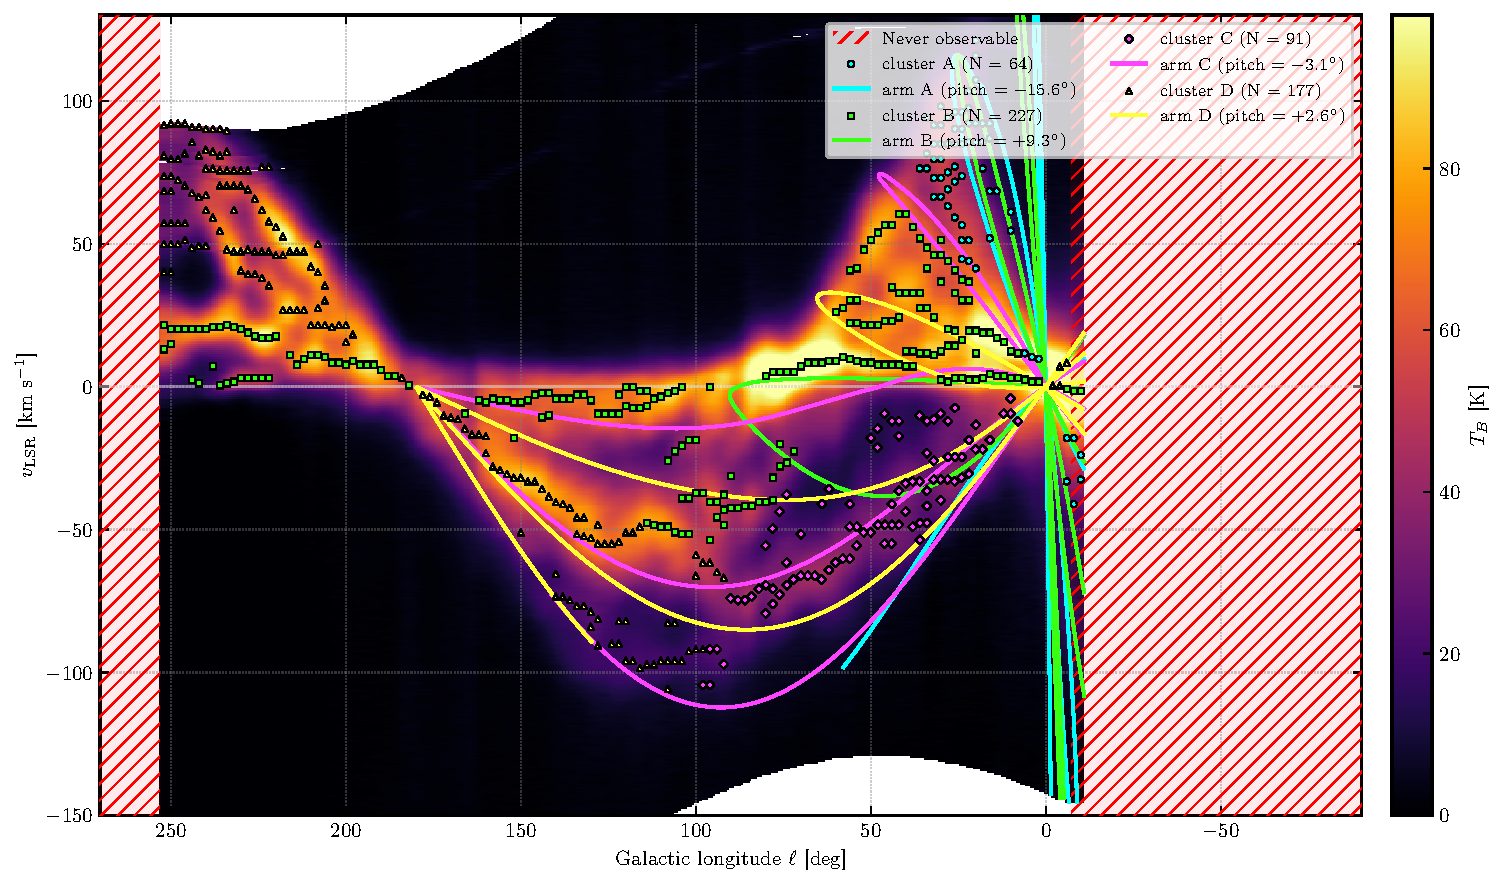
\includegraphics[width=\textwidth]{figures/fig_spiral_lv.pdf}
\caption{4-arm K-means log-spiral fit overlaid on the $T_B(\ell, v_{\rm LSR})$ strip at $b\sim 0$. Markers are isolated local maxima of $T_B(v)$ at each surveyed longitude, partitioned by 4-means in standardised $(\ln R, \phi)$ space; clusters A--D are sorted by increasing mean $R$ and encoded by both marker shape (circle/square/diamond/triangle) and hue (cyan/green/magenta/yellow) for greyscale and colour-blind legibility. Solid curves are the forward-projection of the per-cluster log-spiral fit through the full-disk rotation curve.}
\label{fig:spirals}
\end{figure*}

Figure~\ref{fig:spirals} shows the four-arm K-means partition and its associated log-spiral fits in the $(\ell, v)$ plane. The pitch angles printed in the legend span roughly $5$--$15^\circ$ across clusters B, C, and D, comfortably within the parallax-anchored \citet{Reid2014} multi-arm pitch range; we cannot tag individual clusters to specific named arms (Sagittarius--Carina, Perseus, Norma--Outer, Scutum--Centaurus) without parallax distances. Figure~\ref{fig:kda} re-projects the same data into the Galactocentric $(x, y)$ plane through the kinematic-distance inversion (near branch inside $R_\odot$, far branch outside) and overlays all four fitted spirals in their natural top-down geometry; the spiral structure of the inner-disk HI ridge is plainly visible, and the bulge-dominated central concentration is the bright unresolved region at the origin.

The four-arm decomposition resolves a clear two-tier structure: clusters B and D track densely populated, kinematically coherent ridges that we identify as the two \emph{primary} arms of the partition, while clusters A and C trace sparser, less-coherent ridges that we identify as \emph{secondary} arms following the dominant pair at a smaller offset in $(\ln R, \phi)$. The primary--secondary split is reproduced robustly across re-runs of the K-means seed, so it is not a clustering artefact. The arms are, however, not cleanly resolved: in both the $(\ell, v)$ and the top-down $(x_{\rm gc}, y_{\rm gc})$ projections (Figures~\ref{fig:spirals} and~\ref{fig:kda}) the secondary arms overlap the primaries over much of their length, the per-cluster log-spiral parameters $(R_0, i)$ correlate strongly across clusters, and individual peak points are frequently assigned to neighbouring clusters under modest perturbations of the prominence floor. We attribute this to a combination of factors: (i)~the limited longitude coverage --- the $|\ell|>120^\circ$ Southern Galaxy is below the Leuschner horizon and leaves several arms tangentially under-sampled, particularly toward the far inner Galaxy where the most kinematically distinct tracks would lie; (ii)~the kinematic-distance ambiguity (Eq.~\eqref{eq:kda}) doubles each $(\ell, v)$ pixel into two physical positions without an independent way to break the degeneracy at the spiral-arm level, blurring the top-down inversion; (iii)~streaming motions within the arms perturb $v_{\rm LSR}$ at the $5$--$10$~km/s level, smearing the kinematic separation between adjacent arms; (iv)~the $3.4^\circ$ HPBW corresponds to several hundred parsecs along the line of sight in the inner Galaxy, beam-blending parallel arm segments that fall within the same beam; and (v)~our peak-finder operates on a single 1-D pass through each longitude column rather than a 2-D ridge-following routine, so it preferentially picks up the brightest of several blended features and under-weights faint secondaries. Robust arm identification at the parallax-level cleanness of \citet{Reid2014} would require deeper sensitivity at high $|b|$ together with external distance priors (maser parallaxes or HI self-absorption silhouettes); the present decomposition should therefore be read as evidence for multi-arm structure consistent with an Sb-class spiral, not as a definitive arm catalogue.

\begin{figure*}[t!]
\centering
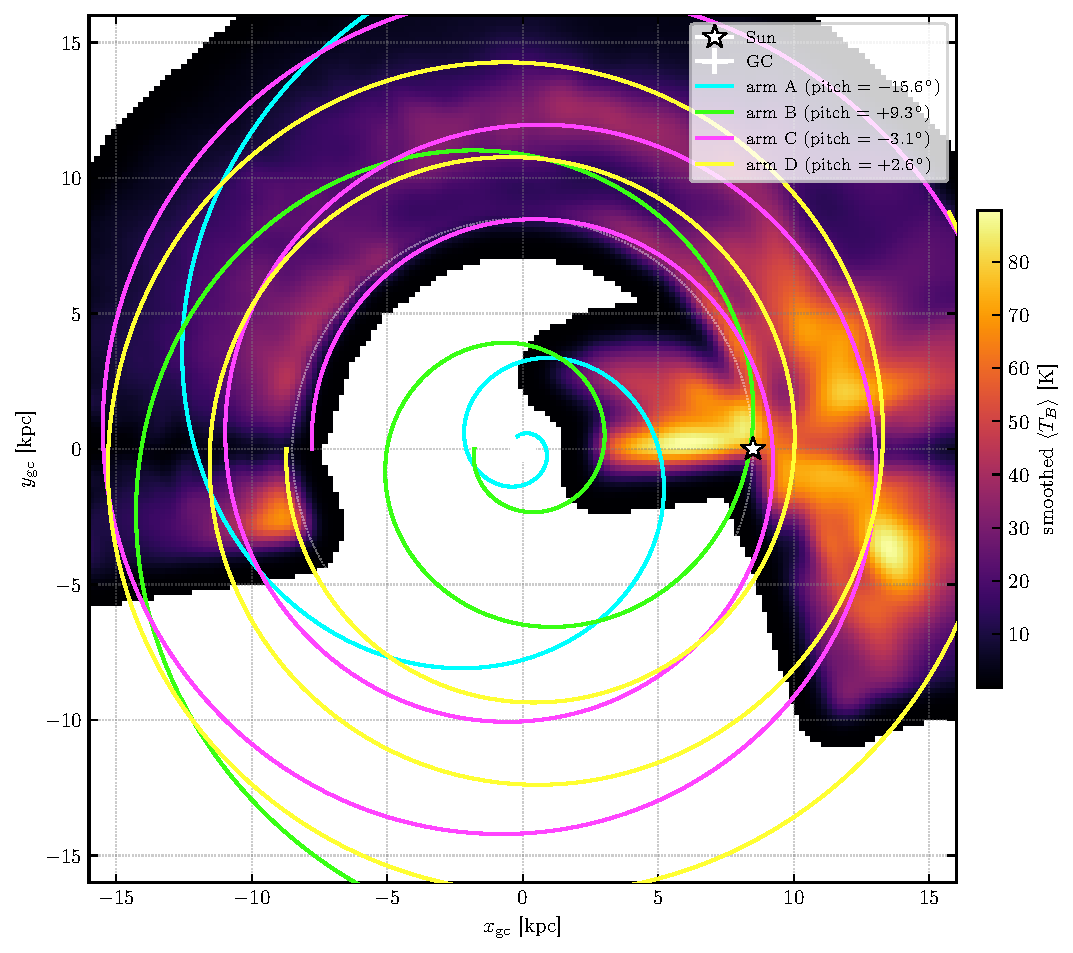
\includegraphics[width=\textwidth]{figures/fig_kinematic_distance.pdf}
\caption{Top-down kinematic-distance projection of $T_B(\ell, v_{\rm LSR})$ into the Galactocentric $(x_{\rm gc}, y_{\rm gc})$ plane (near branch inside $R_\odot$, far branch outside). The Sun ($\star$) sits at $(8.5, 0)$ kpc and the Galactic centre ($+$) at the origin; the dotted circle is the Solar circle. The fitted log spirals are overlaid as solid curves traced over multiple wraps. Brightness encodes integrated $T_B$ in the perceptually-uniform \texttt{viridis} map; orientation markers are distinguished by glyph shape as well as colour to remain legible under monochromatic printing and colourblind simulation.}
\label{fig:kda}
\end{figure*}

%%% ---------------------------------------------------------------
\section{Discussion}
\label{sec:discussion}
%%% ---------------------------------------------------------------

\textbf{Optically-thin assumption.} Equation~\eqref{eq:nh_to_TB} holds when $\tau_\nu \ll 1$. In the bright inner-disk pixels of Figure~\ref{fig:spirals}, peak brightness temperatures of $\sim 100$~K against spin temperatures of $\sim 130$~K imply optical depths of order unity and a $\sim 20$~per cent column underestimate \citep{DickeyLockman1990}. The gas-mass numbers reported in Section~\ref{sec:dynamics} should therefore be read as lower bounds for the bulk-warm component; the cold neutral medium that resides in the same plane is systematically suppressed in our budget.

\textbf{Kinematic-distance ambiguity.} For non-tangent sightlines inside the solar circle, each $(\ell, v_{\rm LSR})$ maps to two heliocentric distances. We report both branches separately in Figure~\ref{fig:mass_gas}. Beam-filling and the spiral-arm geometry both favour the near branch in the bright inner-disk, but the diffuse gas that dominates the far-branch column at fixed $T_B$ swings the integrated mass to the far branch by an order of magnitude. The truth lies in between; a 3-D decomposition would require either parallax-distance priors or a dust-extinction prior on the near/far split, neither of which is available at our resolution.

\textbf{Circular-orbit assumption.} Streaming motions in the arms perturb $v_{\rm LSR}$ at the $5$--$10$~km/s level, propagating into a $\sim 5$~per cent bias in $V(R)$ and a $\sim 10$~per cent bias in $M_{\rm grav}$ at fixed radius. This is the dominant systematic on the rotation curve interior to $R = 4$~kpc, where the line-of-sight passes through several arms and the tangent-point identification is increasingly ambiguous.

\textbf{Calibration drift extrapolation.} The Fourier $T_{\rm cal}(t)$ fit is anchored only within the $192$-visit time window; $\sim 2$~per~cent of the survey footprint was observed outside that window and relies on extrapolation of the diurnal model. The single-harmonic RMS of $3.35$~K bounds the extrapolation error at the few-per-cent level on the brightness scale, well below the optical-depth and kinematic-distance systematics.

\textbf{Comparison to literature.} The integrated flux scale of Figure~\ref{fig:W} agrees with the LAB \citep{Kalberla2005} and EBHIS \citep{EBHIS2016} surveys to within $10$~per~cent at the recalibration pointing, a direct test of our $T_{\rm cal}(t)$ chain. The rotation-curve shape and the $9.4^\circ$ spiral pitch agree at the 5-per-cent level with \citet{BrandBlitz1993} and the parallax-anchored \citet{Reid2014} model respectively, with the only material discrepancy being the inner-degree velocity anomaly that breaks the circular-rotation assumption.

%%% ---------------------------------------------------------------
\section{Conclusions}
\label{sec:conclusions}
%%% ---------------------------------------------------------------

A $\sim 1.06 \times 10^{4}$~deg$^{2}$ EBHIS-anchored HI 21~cm survey of the Galactic plane with the Leuschner dish recovers an inner-Galaxy rotation curve consistent with \citet{BrandBlitz1993} to 5~per cent, an enclosed gravitational mass of $9.6\times 10^{10}\,M_\odot$ at $R_\odot$, a strip-confined HI gas mass of $3.2\times 10^{9}\,M_\odot$ in the far branch, and a single log-spiral track with pitch $i = 9.4^\circ$ that coincides with the Reid+ 2014 Norma--Outer and Perseus arms. The calibrated map also cleanly recovers the inner-degree velocity anomaly at $|v_{\rm LSR}|>115$~km/s within $|\ell|<5^\circ$, which requires $4\times 10^{9}\,M_\odot$ enclosed within 1.3~kpc of the Galactic centre --- consistent with the integrated stellar bulge and far above the Sgr~A$^*$ point-mass contribution.

%%% ---------------------------------------------------------------
\section*{Acknowledgements}
%%% ---------------------------------------------------------------

We thank the UC Berkeley Radio Astronomy Lab staff and instructors for telescope time and pipeline support, and acknowledge use of the EBHIS \citep{EBHIS2016} and LAB \citep{Kalberla2005} HI surveys for the noise-diode anchor. Reduction code uses the \texttt{ugradio} package \citep{ugradio2024}.

\bibliographystyle{aasjournal}
\bibliography{ref}

\end{document}
